\documentclass{beamer}

\usepackage[mode=buildnew,subpreambles=true]{standalone}
%%%% PACKAGES

\usepackage{import}
\usepackage[toc,page]{appendix}
\usepackage[T1]{fontenc}
\usepackage[english]{babel}
\usepackage[utf8]{inputenc}
\usepackage{graphicx}
\usepackage{adjmulticol}
\usepackage[labelfont=bf]{caption}
\usepackage{float}
\usepackage{graphicx}
\usepackage{subcaption}
\usepackage{fancyhdr}
\usepackage{url}
\usepackage{amsmath} % collection de symboles mathématiques
\usepackage{amssymb} % collection de symboles mathématiques
\usepackage{amsthm}
\usepackage{bbm}
\usepackage{bm}
\usepackage{stmaryrd}
\usepackage{mathtools}
\usepackage{cancel}
\usepackage{titling}
\usepackage{nameref} % pour désigner des parties par leur nom
\usepackage{url} % pour mettre des URL
\usepackage{cite}
% \usepackage[sectionbib]{chapterbib}
% \usepackage{chapterbib}
\usepackage[numbers,sort&compress]{natbib}
% \usepackage[square,numbers,sectionbib]{natbib}
% \usepackage{bibunits}
% \usepackage{biblatex}
\usepackage{tabularx}
\usepackage{titlesec, blindtext, color}
% \usepackage{auto-pst-pdf}

%%%% TIKZ

\usepackage{pgf, tikz}
\usetikzlibrary{shapes.misc}
\usetikzlibrary{decorations.pathreplacing}

\tikzset{cross/.style={cross out, draw=black, minimum size=2*(#1-\pgflinewidth), inner sep=0pt, outer sep=0pt},
%default radius will be 1pt.
cross/.default={0.25pt},
    point/.style={
    thick,
    draw=black,
    cross out,
    inner sep=0pt,
    minimum width=4pt,
    minimum height=4pt,
    },
}

%%%% STYLE

\textheight=25 true cm
\textwidth= 20. true cm
\oddsidemargin=-1.75truecm
\evensidemargin=0.5truecm
\topmargin=-3 truecm

% \setlength{\topmargin}{-1cm}
% \setlength{\headheight}{0.43cm}
% \setlength{\headsep}{0.8cm}
% \setlength{\footskip}{0cm}
% \setlength{\textwidth}{17cm}
% \setlength{\textheight}{23.5cm}
% \setlength{\voffset}{-2.5cm}
% \setlength{\hoffset}{-0.25cm}
% \setlength{\oddsidemargin}{0cm}
% \setlength{\evensidemargin}{0cm}
\setlength{\parindent}{0pt}
\setlength{\footskip}{1.5cm}

\setlength{\droptitle}{-1cm}

\setcounter{tocdepth}{3}
\setcounter{secnumdepth}{3}

\definecolor{lcolor}{rgb}{0,0,0.6} % définition de la couleur des liens pdf
\usepackage{hyperref}
\hypersetup{pdftex,colorlinks=true,
linkcolor=lcolor,
citecolor=lcolor,
urlcolor=lcolor,
hyperindex=true,
hyperfigures=false} % fichiers pdf 'intelligents', avec des liens entre les références, etc.

\definecolor{gray75}{gray}{0.75}

\AtBeginDocument{\addtocontents{toc}{\protect\thispagestyle{empty}}}

% \titleformat{\chapter}[hang]{\vspace{-50pt}\huge\bfseries}{\thechapter\hspace{20pt}\textcolor{gray75}{|}\hspace{20pt}}{0pt}{\huge\bfseries}
\titleformat{\subsection}[block]{\hspace{0em}}{\large\textbf\thesubsection}{1em}{\large\textbf}
\titleformat{\subsubsection}[block]{\hspace{0em}}{\Small\textbf\thesubsubsection}{1em}{\Small\textbf}

\usepackage{etoolbox}
\makeatletter
\patchcmd{\@chap@pppage}{\thispagestyle{plain}}{\thispagestyle{empty}}{}{}
\makeatother

\captionsetup{font=normalsize}
\captionsetup[sub]{font=scriptsize}

%%%% COMMANDS

\providecommand{\ie}{\textit{i.e.}~}

%\renewcommand*\thesection{\arabic{section}}

\makeatletter
\providecommand*\bigcdot{\mathpalette\bigcdot@{.5}}
\providecommand*\bigcdot@[2]{\mathbin{\vcenter{\hbox{\scalebox{#2}{$\m@th#1\bullet$}}}}}
\makeatother

\providecommand{\appropto}{\mathrel{\vcenter{
  \offinterlineskip\halign{\hfil$##$\cr
    \propto\cr\noalign{\kern2pt}\sim\cr\noalign{\kern-2pt}}}}}

\providecommand\encircle[1]{%
  \tikz[baseline=(X.base)]
    \node (X) [draw, shape=circle, inner sep=0] {\strut #1};}

\providecommand\phantomarrow[2]{%
  \setbox0=\hbox{$\displaystyle #1\to$}%
  \hbox to \wd0{%
    $#2\mapstochar
     \cleaders\hbox{$\mkern-1mu\relbar\mkern-3mu$}\hfill
     \mkern-7mu\rightarrow$}%
  \,}

\providecommand{\myparagraph}[1]{\paragraph{#1}\mbox{}\\\vspace{-5pt}}

\providecommand{\isEquivTo}[1]{\underset{#1}{\sim}}

\makeatletter
\providecommand{\subalign}[1]{%
  \vcenter{%
    \Let@ \restore@math@cr \default@tag
    \baselineskip\fontdimen10 \scriptfont\tw@
    \advance\baselineskip\fontdimen12 \scriptfont\tw@
    \lineskip\thr@@\fontdimen8 \scriptfont\thr@@
    \lineskiplimit\lineskip
    \ialign{\hfil$\m@th\scriptstyle##$&$\m@th\scriptstyle{}##$\crcr
      #1\crcr
    }%
  }
}
\makeatother

% \makeatletter
% % Original \l@section:
% %\renewcommand*\l@section{\vskip 6pt plus 1pt minus 1pt
% %                         \@dottedtocline{1}{1.5em}{2.3em}}
% % Modified \l@section:
% \renewcommand*\l@section{\ifnum\c@tocdepth>\z@\vskip 6pt plus 1pt minus 1pt \fi
%                          \@dottedtocline{1}{1.5em}{2.3em}}
% \makeatother

\providecommand\smallO[1]{
      \mathchoice
         {% mode \displaystyle
            \ensuremath{\mathop{}\mathopen{}{\scriptstyle\mathcal{O}}\mathopen{}\left(#1\right)}
         }
         {% mode \textstyle
            \ensuremath{\mathop{}\mathopen{}{\scriptstyle\mathcal{O}}\mathopen{}\left(#1\right)}
         }
         {% mode \scriptstyle
            \ensuremath{\mathop{}\mathopen{}{\scriptscriptstyle\mathcal{O}}\mathopen{}\left(#1\right)}
         }
         {% mode \scriptscriptstyle
            \ensuremath{\mathop{}\mathopen{}{o}\mathopen{}\left(#1\right)}
         }
   }

%%%% PATCH

% \makeatletter
% \let\orig@document\document
% \let\orig@enddocument\enddocument
% \def\sa@document{%
%   \endgroup
%   \global\let\enddocument\sa@enddocument
%   \sa@atbegindocument
% }
% \def\sa@enddocument{%
%   \sa@atenddocument
%   \global\let\document\orig@document
%   \global\let\enddocument\orig@enddocument
%   \begingroup
%   \@ignoretrue
%   \def\@currenvir{document}%
%   \aftergroup\endinput
% }
% \makeatother


%%%%% INFORMATION

\title{Collective motion in large deviations of active particles}
\shorttitle{Large deviations of active particles (\href{https://arxiv.org/abs/2009.07112}{arXiv:2009.07112})}

\author{Yann-Edwin Keta}

\location{}

\supervisor{Robert Jack and Frédéric van Wijland}

\date{21/09/2020}

%%%%% DOCUMENT

\begin{document}

%% TITLE PAGE

{
\setbeamertemplate{footline}{}
\makeatletter
    \setbeamertemplate{headline}[default]
    \def\beamer@entrycode{\vspace*{-\headheight}}
\begin{frame}[noframenumbering]

\vspace*{-4mm}
{
 \hspace*{-\beamerleftmargin}%
\begin{minipage}{\paperwidth}
\includegraphics[width=\paperwidth]{header.eps}
\end{minipage}
}

\titlepage

% \vspace{-10pt}
\begin{center}
{\bf\large \href{https://arxiv.org/abs/2009.07112}{arXiv:2009.07112}}\\
\vspace{10pt}
\href{https://github.com/yketa/DAMTP_MSC_2019_Wiki}{\footnotesize \faGithub~ yketa/DAMTP\_MSC\_2019\_Wiki}
\end{center}

\end{frame}
}

%% TABLE OF CONTENTS

{\footerwithoutframenumber
\begin{frame}<beamer>[noframenumbering]{Contents}
  \tableofcontents
\end{frame}
}

%% PRESENTATION

\section{Model and methods}

\subsection{Active Brownian particles}

\begin{frame}{Active Brownian particles}

\begin{center}
\begin{tabularx}{\textwidth}{ >{\setlength\hsize{0.13\hsize}}X X }
  {\bf ABP} & $\begin{aligned}
\dot{\boldsymbol{r}}_i &= v_0 \begin{pmatrix} \cos\theta_i \\ \sin\theta_i \end{pmatrix} - \mu \nabla_i U + \sqrt{2 D} \boldsymbol{\eta}_i\\
\dot{\theta}_i &= \sqrt{2 D_r} \xi_i\\
\left<\eta^{\alpha}_i(t) \eta^{\beta}_j(t^{\prime})\right> &= \delta_{\alpha\beta} \delta_{ij} \delta(t - t^{\prime})\\
\left<\xi_i(t) \xi_j(t^{\prime})\right> &= \delta_{ij} \delta(t - t^{\prime})\\
\left<\boldsymbol{u}(\theta_i(t)) \cdot \boldsymbol{u}(\theta_j(t^{\prime}))\right> &= \delta_{ij} e^{-D_r |t - t^{\prime}|}
\end{aligned}$\mbox{}\\\\
{\bf WCA} & $\begin{aligned}
  U = \varepsilon \sum_{1 \leq i < j \leq N} \left[4\left((r_{ij}/\sigma)^{-12} - (r_{ij}/\sigma)^{-6}\right) + 1\right] \Theta(2^{1/6} - r_{ij}/\sigma)\\
\end{aligned}$\\
&\begin{itemize}
\item length: $\sigma = 1$, energy: $\varepsilon = 1$, time: $\sigma/v_0 = 1$
\item $\mu = D/\varepsilon$, $D_r = 3 D/\sigma^2$
\item $\phi = N \pi \sigma^2/(4 L^2) = 0.65$, $\tilde{l}_{\rm p} = v_0/(\sigma D_r)$
\end{itemize}
\end{tabularx}
\end{center}
\vspace{-10pt}

\footfullcitenomark{nemoto2019optimizing}

\end{frame}

\subsection{Large deviations of active work}

\begin{frame}[t]{Active work}

\vspace{-22pt}

\begin{align*}
\text{\bf instantaneous dissipated power:}~ \dot{\mathcal{W}} = \sum_{i} \dot{\boldsymbol{r}}_i \circ \frac{1}{D} \left(\dot{\boldsymbol{r}}_i - \sqrt{2D} \boldsymbol{\eta}_i\right)
\end{align*}

\pause

\begin{align*}
&\frac{1}{\tau} \int_0^{\tau} \dot{\mathcal{W}}(t) \, \mathrm{d}t = \frac{N v_0^2}{D}  w_{\tau}  + \frac{1}{\tau} [ U(\tau) - U(0) ]\\
&\begin{aligned}w_\tau &= \frac{1}{v_0 N\tau} \sum_{i=1}^N \int_0^\tau \boldsymbol{u}(\theta_i) \circ \mathrm{d}\boldsymbol{r}_i \qquad \text{\bf (active work)}\\
&= 1 + \underbrace{\frac{-D}{v_0 N \tau} \sum_{i=1}^N \int_0^{\tau} \boldsymbol{u}(\theta_i) \circ \nabla_i U \, \mathrm{d} t}_{\displaystyle w_{f, \tau}} + \underbrace{\frac{1}{v_0 N \tau} \sum_{i=1}^N \int_0^{\tau} \boldsymbol{u}(\theta_i) \circ \sqrt{2 D} \boldsymbol{\eta}_i \, \mathrm{d}t}_{\displaystyle w_{\eta, \tau}}
\end{aligned}
\end{align*}

\pause

\hfill
\begin{minipage}{0.4\linewidth}
\centering
\bf Flocking
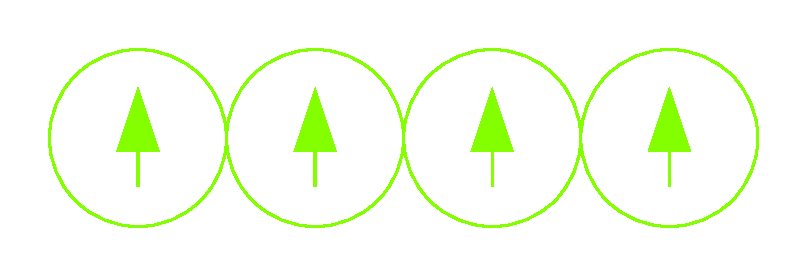
\includegraphics[width=\linewidth]{w1.eps}
$\nabla U_{ij} = 0 \Rightarrow w_{\tau} \approx 1$
\end{minipage}
\hfill
\begin{minipage}{0.4\linewidth}
\centering
\bf Jamming
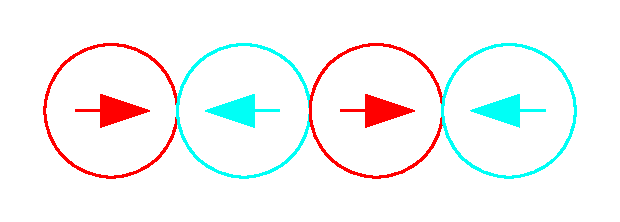
\includegraphics[width=\linewidth]{w0.eps}
$\dot{\boldsymbol{r}}_i \approx 0 \Rightarrow w_{\tau} \approx 0$
\end{minipage}
\hfill\hfill

\end{frame}

\begin{frame}[t]{Biased ensemble}

\begin{align*}
\text{\bf biased average:}~\left<\mathcal{A}\right>_s = \frac{\left<\mathcal{A} e^{-s N \tau w_{\tau}}\right>}{\left<e^{-s N \tau w_{\tau}}\right>} \only<2->{=\frac{\left<\mathcal{A} e^{-s N \tau w_{f, \tau}}\right>_{v^{\rm con}_s}}{\left<e^{-s N \tau w_{f, \tau}}\right>_{v^{\rm con}_s}}}
\end{align*}

\only<2->{
\begin{align*}
v^{\rm con}_s = v_0 \left(1 - \frac{2 s D}{v_0^2}\right)\
\end{align*}
\only<3->{

\begin{align*}
w^{\rm free}(s) = \left<w_{\tau}\right>_{s, U=0} = 1 - \frac{2 s D}{v_0^2}
\end{align*}
\begin{align*}
s^{\rm con} = s \left(1 - \frac{2 s D}{v_0^2}\right),~ s w_{f, \tau} = s^{\rm con} \frac{w_{f, \tau}}{w_{free}(s)}
\end{align*}
}
}

\end{frame}

\begin{frame}{Cloning algorithm}

\vspace{-10pt}
\begin{align*}
Z_{\tau}(s) = \left<e^{-s N \tau w_{\tau}}\right> \equiv \begin{split}&\text{{\it dynamical} partition function}\\ &\text{of a Boltzmann-like measure}\end{split}
\end{align*}

\pause
\begin{itemize}
  \item[$\Rightarrow$] \textit{Cloning algorithm}: simulate $n_c \gg 1$ copies of the system and clones/deletes them at regular intervals to enforce biased measure.
\end{itemize}

\begin{figure}
\centering
\includegraphics[width=0.45\textwidth]{Nemoto_2016_fig1a.png}
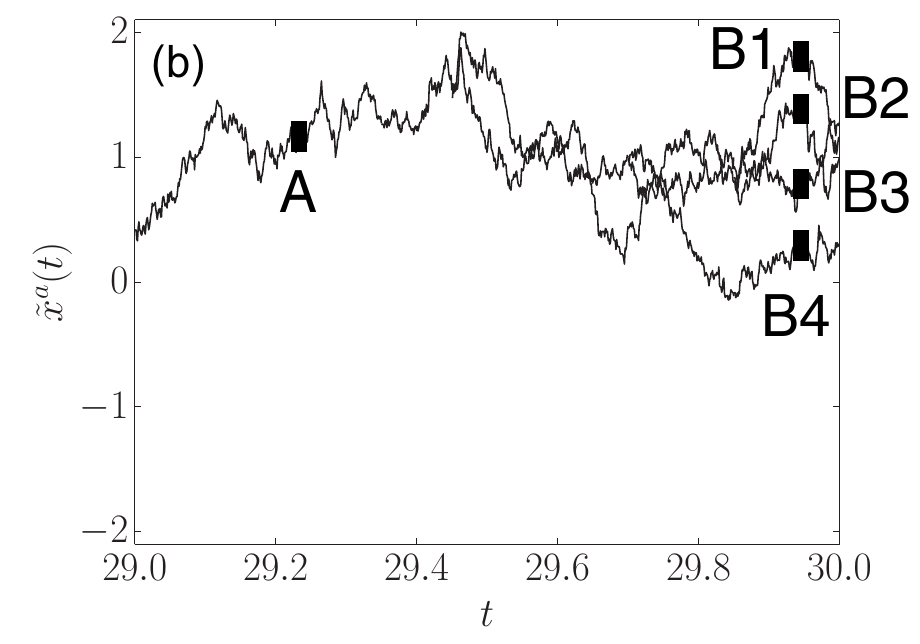
\includegraphics[width=0.45\textwidth]{Nemoto_2016_fig1b.png}
\caption{$Z_{\tau}(s) = \left<\exp\left(s \int_0^{\tau} x(t)(1 + x(t)) \, \text{d}t\right)\right>$, $s = 1$. \FigureFrom{nemoto2016population}{}}
\end{figure}

\end{frame}

\section{2 RTPs on a ring}

\begin{frame}{Run-and-tumble particles on a ring}

\vspace{-5pt}

\begin{center}
\begin{tabularx}{\textwidth}{ >{\setlength\hsize{0.26\hsize}}X X }
  {\bf RTP} & \begin{tabular}{l} $\dot{r}_i = \alpha_i v_0 - \frac{\partial}{\partial r_i} V(r_{12})$ \\ tumble ($\alpha_i \to -\alpha_i$) rate: $\tau_{\rm p}^{-1}$ \\ ring length: $L$, persistence length: $l = v_0 \tau_{\rm p}$ \end{tabular}\mbox{}\\\\
{\bf potential} & \begin{tabular}{cc} \begin{tabular}{l} $\lim_{r_{12} \to 0} V(r_{12}) = \infty$ \\ $V(r_{12} > \varepsilon) = 0$ \\ $\frac{\partial}{\partial r_1} V(r_{12} = r^*) = -v_0$ \end{tabular} & \begin{tabular}{l} hard core limit: \\ $\varepsilon \to 0$, $r^* \to 0$ \end{tabular} \end{tabular}\mbox{}\\\\
{\bf active work} & \begin{tabular}{l} $\dot{w}^{\rm RTP}_f = v_0 (\alpha_1 - \alpha_2) \frac{\partial}{\partial r_1} V(r_{12}) = \begin{cases} - 2 v_0^2 &\text{ if contact} \\ 0 &\text{ otherwise} \end{cases}$ \\ $\left<\mathcal{A}\right>_{\lambda} = \frac{\left<\mathcal{A} e^{-\lambda \int_0^{\tau} \dot{w}^{\rm RTP}_f(t) \, \mathrm{d}t}\right>}{\left<e^{-\lambda \int_0^{\tau} \dot{w}^{\rm RTP}_f(t) \, \mathrm{d}t}\right>}$ \end{tabular}\mbox{}\\\\
{\bf polarisation} & \begin{tabular}{l} $\nu^{\rm RTP} = \frac{1 + \alpha_1\alpha_2}{2}$ \end{tabular}
\end{tabularx}
\end{center}

\end{frame}

\begin{frame}{Biased ensemble averages}

\begin{figure}
\centering
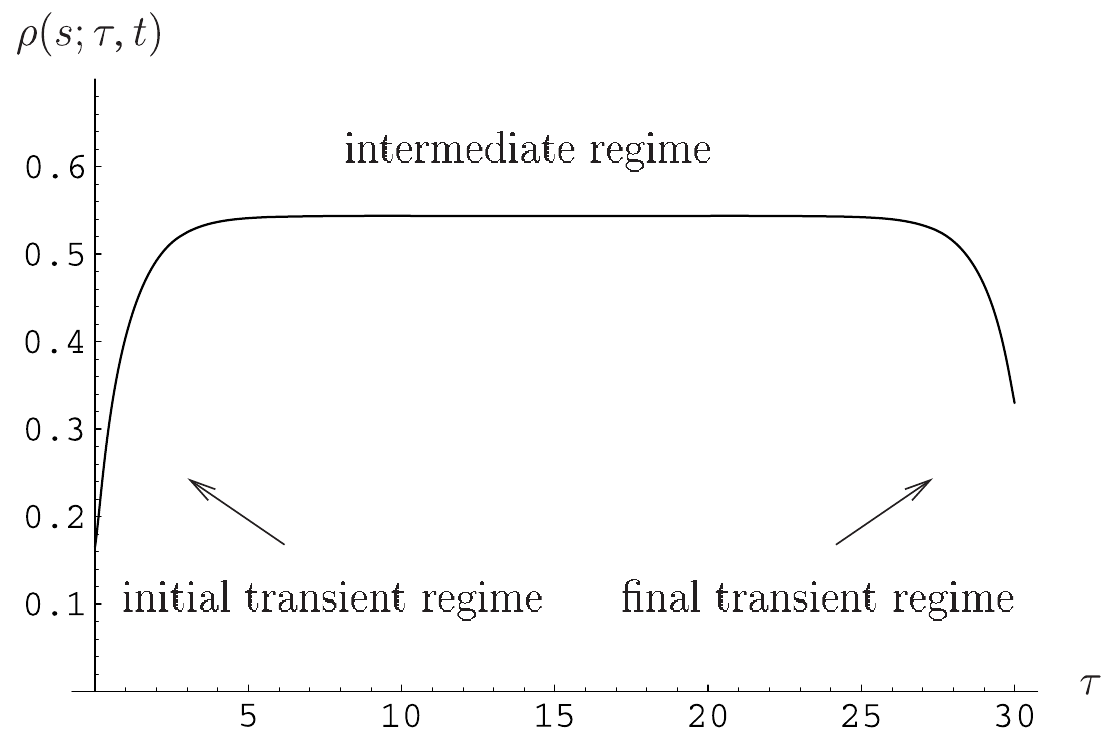
\includegraphics[width=0.45\textwidth]{Garrahan_2009_fig7.png}
\caption{Example trajectory for the $\lambda$-ensemble ($s$-ensembe) of trajectories of length $t = 30$. \FigureFrom{garrahan2009first}{}}
\end{figure}

\begin{center}
\begin{tabular}{c@{\hskip 30pt}c}
{\bf intermediate regime} & {\bf final regime}\mbox{}\\\\
$\nu^{\rm RTP}_{\rm ave}(\lambda) = \lim_{\tau \to \infty} \left<\frac{1}{\tau} \int_0^{\tau} \nu^{\rm RTP}(t) \, \mathrm{d}t\right>_{\lambda}$ & $\nu^{\rm RTP}_{\rm end}(\lambda) = \left<\nu^{\rm RTP}\right>_{\lambda}$
\end{tabular}
\end{center}

\end{frame}

\begin{frame}{Eigenproblem}

\begin{tabularx}{\textwidth}{ >{\setlength\hsize{0.40\hsize}}X X }
{\bf dynamical free energy density:} & $\psi^{\rm RTP}(\lambda) = \lim_{\tau \to \infty} \frac{1}{\tau} \log \left<\exp\left(-\lambda \int_0^{\tau} \dot{w}^{\rm RTP}_f(t) \, \mathrm{d}t\right)\right>$
\end{tabularx}

\begin{align*}
\psi^{\rm RTP}(\lambda) \boldsymbol{P}_{\lambda} = \left(\boldsymbol{\mathcal{L}} - \lambda \dot{w}^{\rm RTP}_f \boldsymbol{I}\right) \boldsymbol{P}_{\lambda} \qquad \psi^{\rm RTP}(\lambda) \boldsymbol{Q}_{\lambda} = \left(\boldsymbol{\mathcal{L}}^{\dagger} - \lambda \dot{w}^{\rm RTP}_f \boldsymbol{I}\right) \boldsymbol{Q}_{\lambda}
\end{align*}
$\boldsymbol{\mathcal{L}}, \boldsymbol{\mathcal{L}}^{\dagger} \equiv$ forward and backward Fokker-Planck operators\\

\begin{align*}
\boldsymbol{P}^{\rm end}_{\lambda} &\equiv P^{\alpha_1\alpha_2}_{\lambda}(r)\\
&= \varepsilon^{\alpha_1\alpha_2}_{\lambda}(r) + \gamma^{\alpha_1\alpha_2,{\rm l}}_{\lambda} \delta(r) + \gamma^{\alpha_1\alpha_2,{\rm r}}_{\lambda} \delta(L - r)\\
\nu^{\rm RTP}_{\rm end}(\lambda) &= \int_0^L (P^{++}_{\lambda}(r) + P^{--}_{\lambda}(r)) \, \mathrm{d}r
\end{align*}
\begin{align*}
\boldsymbol{P}^{\rm ave}_{\lambda} &\equiv \hat{P}^{\alpha_1\alpha_2}_{\lambda}(r) = P^{\alpha_1\alpha_2}_{\lambda}(r) Q^{\alpha_1\alpha_2}_{\lambda}(r)\\
&= \hat{\varepsilon}^{\alpha_1\alpha_2}_{\lambda}(r) + \hat{\gamma}^{\alpha_1\alpha_2,{\rm l}}_{\lambda} \delta(r) + \hat{\gamma}^{\alpha_1\alpha_2,{\rm r}}_{\lambda} \delta(L - r)\\
\nu^{\rm RTP}_{\rm ave}(\lambda) &= \int_0^L (\hat{P}^{++}_{\lambda}(r) + \hat{P}^{--}_{\lambda}(r)) \, \mathrm{d}r
\end{align*}

\end{frame}

\begin{frame}{Polarisation averages}

\begin{figure}
\centering
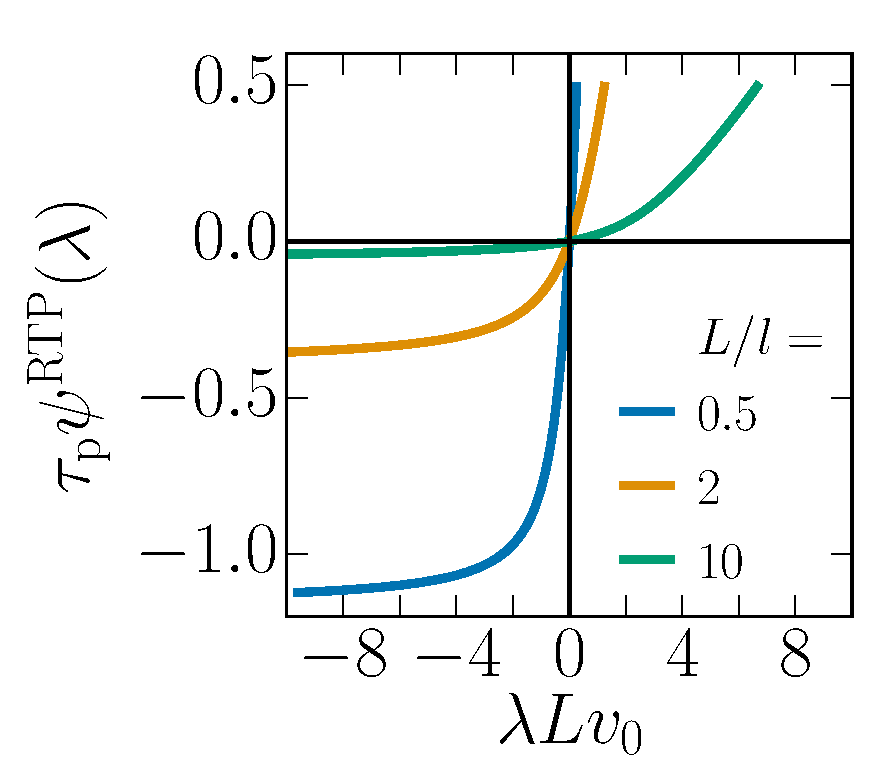
\includegraphics[width=0.45\textwidth]{exactPsiRTP.eps}
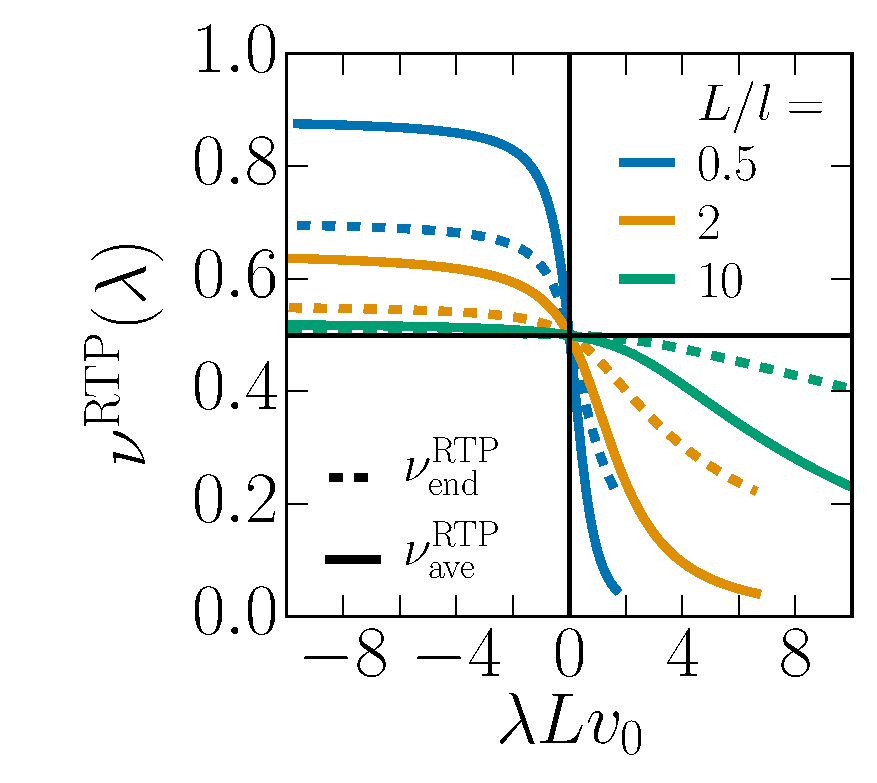
\includegraphics[width=0.45\textwidth]{exactNuRTP.eps}
\caption{{\bf (left)} Dynamical free energy density. {\bf (right)} Polarisation. \FigureFrom{keta2020collective}{}}
\end{figure}

\begin{align*}
- \frac{\partial}{\partial \lambda} \psi^{\rm RTP}(\lambda) = \left<w^{\rm RTP}_f\right>_{\lambda}
\end{align*}

\end{frame}

\section{Large deviations of ABPs}

\subsection{Polarisation}

\begin{frame}{Generating polarised trajectories}

\begin{align*}
\text{\bf polarisation:}~ \hat{\nu} =\left|\frac{1}{N} \sum_{i=1}^N \boldsymbol{u}(\theta_i)\right|,~ \bar{\nu}_{\tau} = \frac{1}{\tau} \int_0^{\tau} \hat{\nu}(t) \, \text{d}t,~ \hat{\nu} e^{\mathrm{i}\varphi} = \frac{1}{N} \sum_{i=1}^N e^{\mathrm{i} \theta_i}
\end{align*}

\begin{figure}
\begin{minipage}{0.55\linewidth}
\centering
\Movie{1}{Nemoto_2019_CM.png}{Nemoto_2019_CM.mp4}
\end{minipage}
\vspace{-15pt}
\caption{\textit{(Movie)} Biased trajectory for $N = 64$, $\phi = 0.65$, $\tilde{l}_{\rm p} = 40$, $s = -3.2$. \FigureFrom{nemoto2019optimizing}{}}
\end{figure}

\end{frame}

\begin{frame}{Modified dynamics}

{\bf modified swim speed:} $\dot{\boldsymbol{r}}_i = {\color{red}v^{\rm con}_s} \boldsymbol{u}(\theta_i) - D \nabla_i U + \sqrt{2 D} \boldsymbol{\eta}_i$\\
{\bf aligning torque:} $\dot{\theta}_i = {\color{red}-D_r \frac{\partial}{\partial \theta_i} \left(- \frac{g N}{D_r} |\boldsymbol{\nu}|^2\right)} + \sqrt{2 D_r} \xi_i$\\
\mbox{}\\

\begin{align*}
P[\{\boldsymbol{r}_i, \theta_i\}] \exp(- s N \tau w_{\tau}) \propto P^{\rm mod}[\{\boldsymbol{r}_i, \theta_i\}] \exp(- s N \tau w^{\rm mod}_{\tau})
\end{align*}
\begin{align*}
s w^{\rm mod}_{\tau} = s \left(1 - \frac{s D}{v_0^2} + w_{f, \tau}\right) - g \left(\frac{1}{N} - \mathcal{I}_{1, \tau} + \frac{g}{D_r} \mathcal{I}_{2, \tau}\right)
\end{align*}

\begin{align*}
\mathcal{I}_{1, \tau} &= \frac{1}{\tau} \int_0^{\tau} |\boldsymbol{\nu}(t)|^2 \, \mathrm{d}t\\
\mathcal{I}_{2, \tau} &= \frac{1}{N \tau} \int_0^{\tau} |\boldsymbol{\nu}(t)|^2 \sum_{i=1}^N \sin(\theta_i(t) - \varphi(t))^2 \, \mathrm{d}t
\end{align*}

\end{frame}

\subsection{Transition to collective motion}

\begin{frame}{Rate function}

{\bf dynamical free energy density:} $\psi(s) = \lim_{\tau \to \infty} \frac{1}{N \tau} \log \left<\exp\left(- s N \tau w_{\tau}\right)\right>$\\
{\bf rate function:} $I(w_{\tau}) = - \lim_{\tau \to \infty} \frac{1}{N \tau} \log P(w_{\tau}) = - w s(w) - \psi(s(w))$\\

\vspace{-5pt}
\begin{figure}
\centering
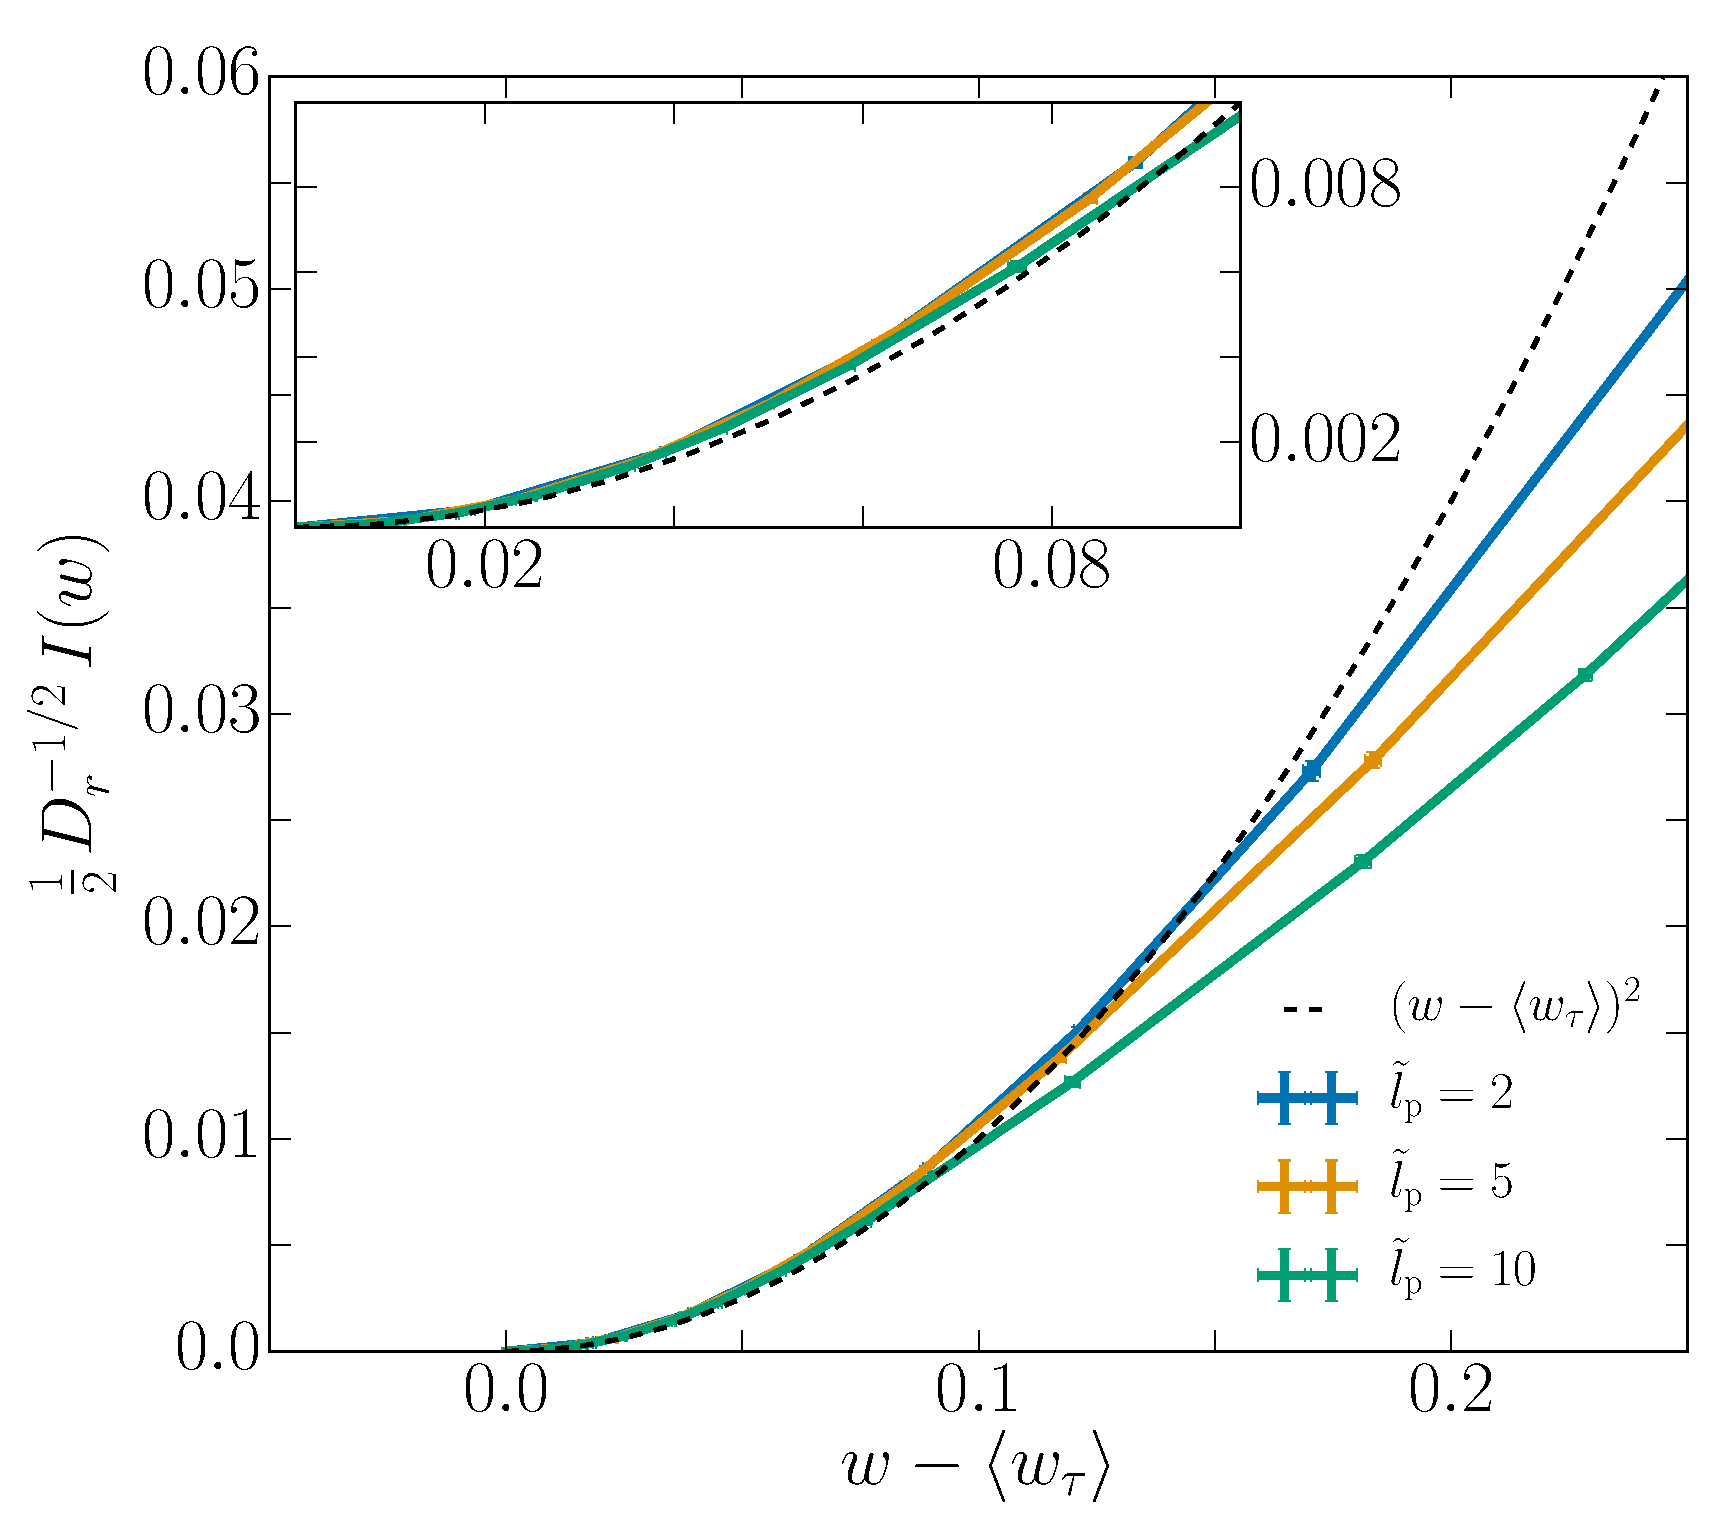
\includegraphics[width=0.45\textwidth]{rate_Nm5000_Dk6500_To1000.eps}
\vspace{-5pt}
\caption{Rate function $I(w)$, $N=50$, $\phi=0.65$, $n_c = 10^3$, $t_{\mathrm{max}} = 10^3$. \FigureFrom{keta2020collective}{}}
\end{figure}

\vspace{-10pt}
\begin{itemize}
  \item[$\Rightarrow$] $\mathrm{Var}(w_{\tau}) \propto D_r^{-1/2}$
\end{itemize}

\end{frame}

\begin{frame}{Relevance of rescaling}

\vspace{-5pt}
\begin{figure}
\centering
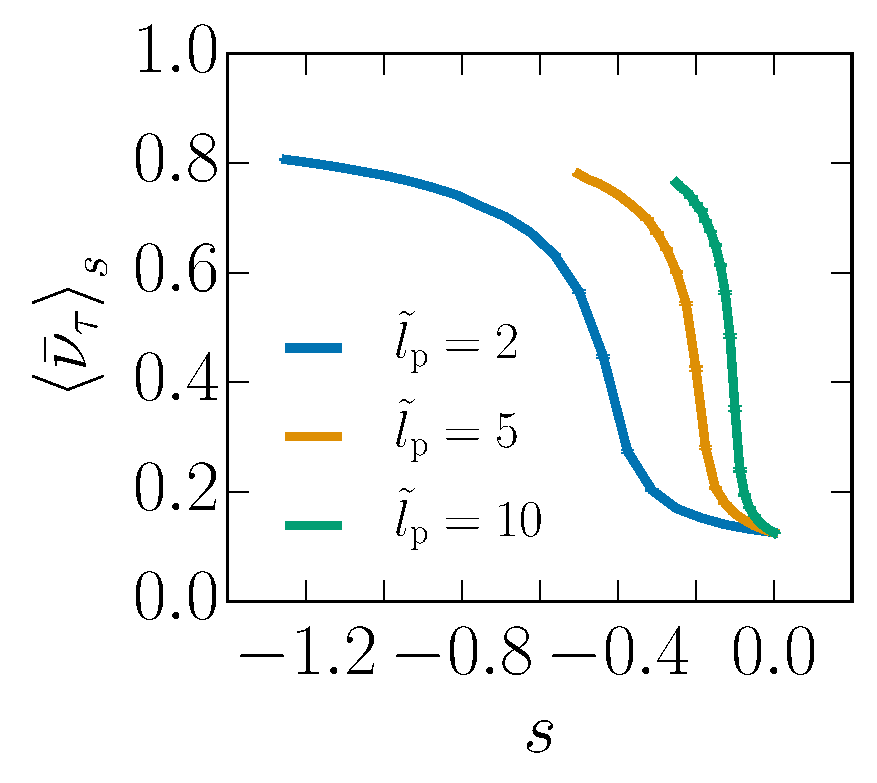
\includegraphics[width=0.35\textwidth]{sOrder_s_Nm5000_Dk6500_To1000.eps}
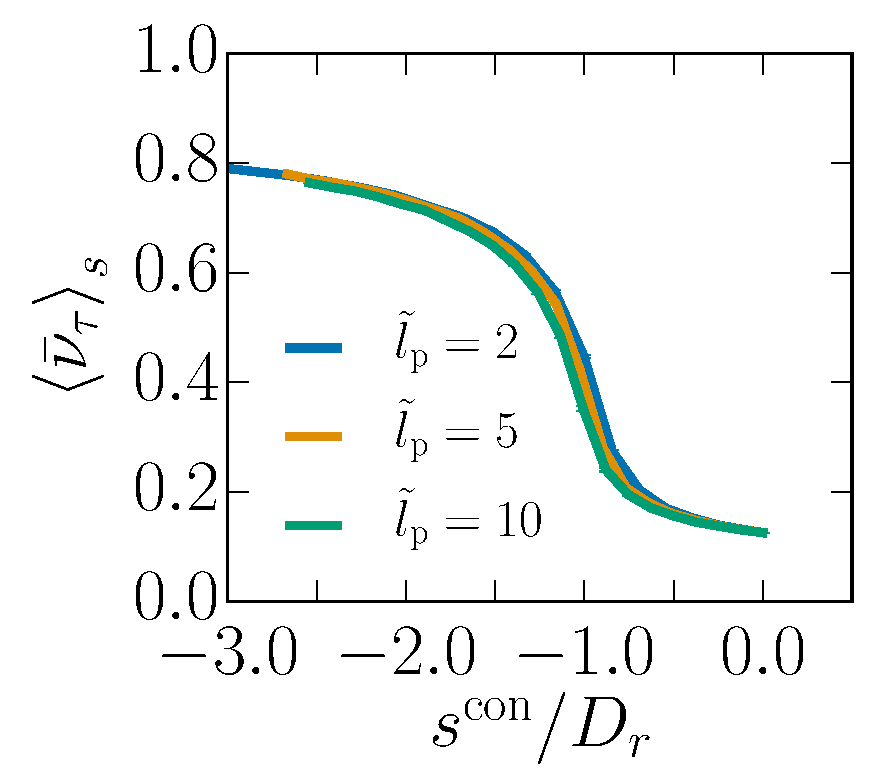
\includegraphics[width=0.35\textwidth]{sOrder_Nm5000_Dk6500_To1000-con.eps}\\
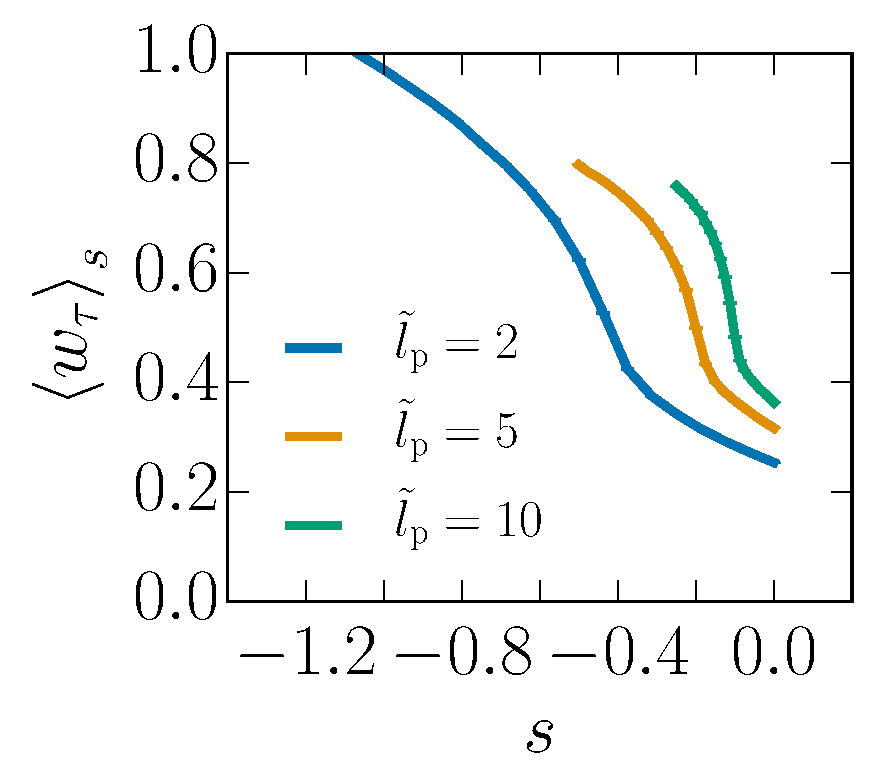
\includegraphics[width=0.35\textwidth]{sWork_s_Nm5000_Dk6500_To1000.eps}
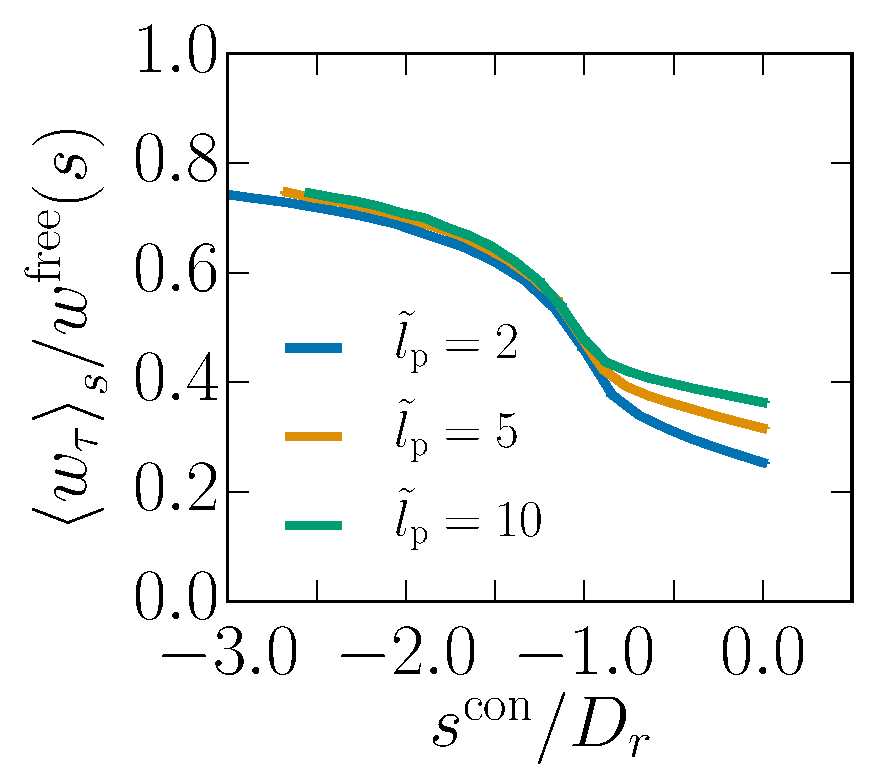
\includegraphics[width=0.35\textwidth]{sWork_Nm5000_Dk6500_To1000-con.eps}
\vspace{-5pt}
\caption{Biased averages of the polarisation $\left<\bar{\nu}_{\tau}\right>_s$ and active work $\left<w_{\tau}\right>_s$, $N = 50$. \FigureFrom{keta2020collective}{}}
\end{figure}

\end{frame}

\begin{frame}{Evidence for dynamical phase transition}

\vspace{-5pt}
\begin{figure}
\centering
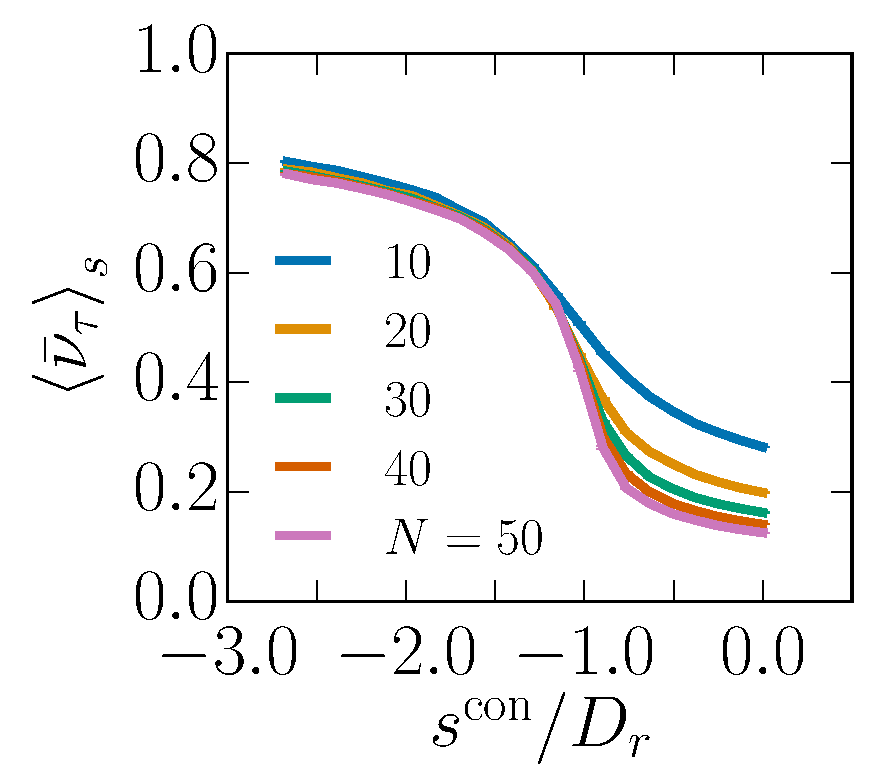
\includegraphics[width=0.45\textwidth]{sOrder_Dk6500_Ll5000_To1000-con.eps}
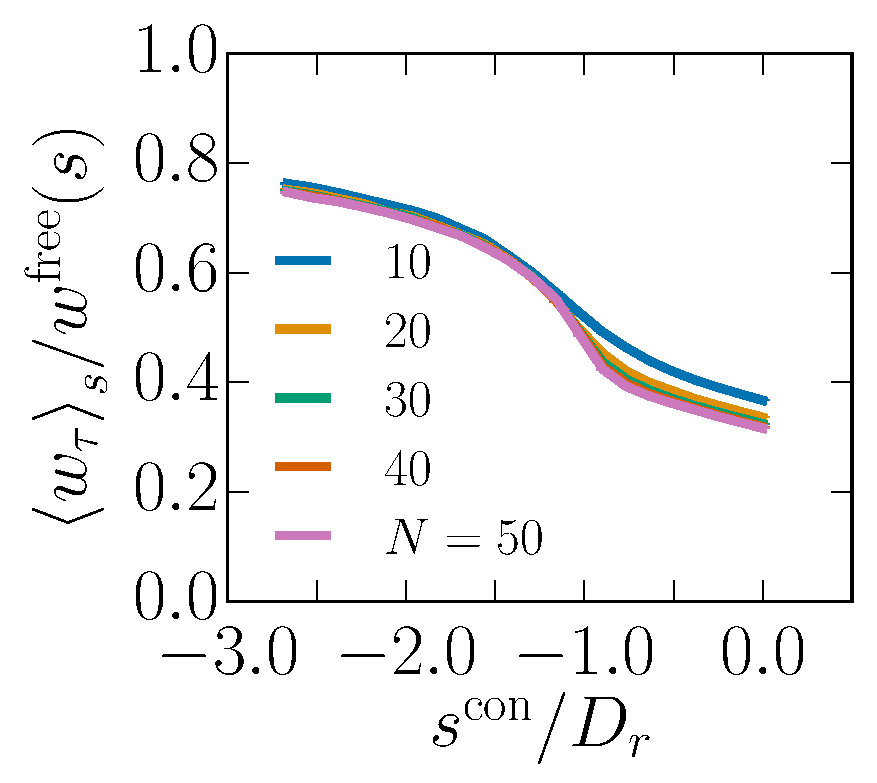
\includegraphics[width=0.45\textwidth]{sWork_Dk6500_Ll5000_To1000-con.eps}
\vspace{-5pt}
\caption{Biased averages of the polarisation $\left<\bar{\nu}_{\tau}\right>_s$ and active work $\left<w_{\tau}\right>_s$, $\tilde{l}_{\rm p} = 5$. \FigureFrom{keta2020collective}{}}
\end{figure}

\begin{itemize}
  \item[$\Rightarrow$] dynamical phase transition at $s^{{\rm con}*} \sim - D_r$
\end{itemize}

\end{frame}

\begin{frame}{Modified dynamics and contraction principle}

{\bf modified swim speed:} $\dot{\boldsymbol{r}}_i = {\color{red}v^{\rm con}_s} \boldsymbol{u}(\theta_i) - D \nabla_i U + \sqrt{2 D} \boldsymbol{\eta}_i$\\
{\bf aligning torque:} $\dot{\theta}_i = {\color{red}-D_r \frac{\partial}{\partial \theta_i} \left(- \frac{g N}{D_r} |\boldsymbol{\nu}|^2\right)} + \sqrt{2 D_r} \xi_i$\\
\mbox{}\\

\begin{align*}
I(w) \leq \lim_{\tau \to \infty} \frac{1}{N \tau} \mathcal{D}_{\rm KL}(P^{\rm mod}_{g(w)} || P)
\end{align*}
\begin{align*}
\mathcal{D}_{\rm KL}(P^{\rm mod}_{g(w)} || P) = \left<\log\frac{P^{\rm mod}_{g(w)}}{P}\right>_{\rm mod}
\end{align*}
\begin{align*}
\lim_{\tau \to \infty} \frac{1}{N \tau} \mathcal{D}_{\rm KL}(P^{\rm mod}_{g(w)} || P) = \left<g(w) \mathcal{I}_{1, \tau} - \frac{g(w)^2}{D_r} \mathcal{I}_{2, \tau}\right>_{\rm mod} - \frac{g(w)}{N}
\end{align*}

\mbox{}\\
\hrule
\mbox{}\\

\begin{align*}
I(w) = \inf_{\nu} I_2(w, \nu) = I_2(w, \nu(w)) \geq \inf_{w^{\prime}} I_2(w^{\prime}, \nu(w))= \mathcal{J}(\nu(w))
\end{align*}

\footfullcitenomark{nemoto2019optimizing}

\end{frame}

\begin{frame}{Bounds to the rate function}

\begin{figure}
\centering
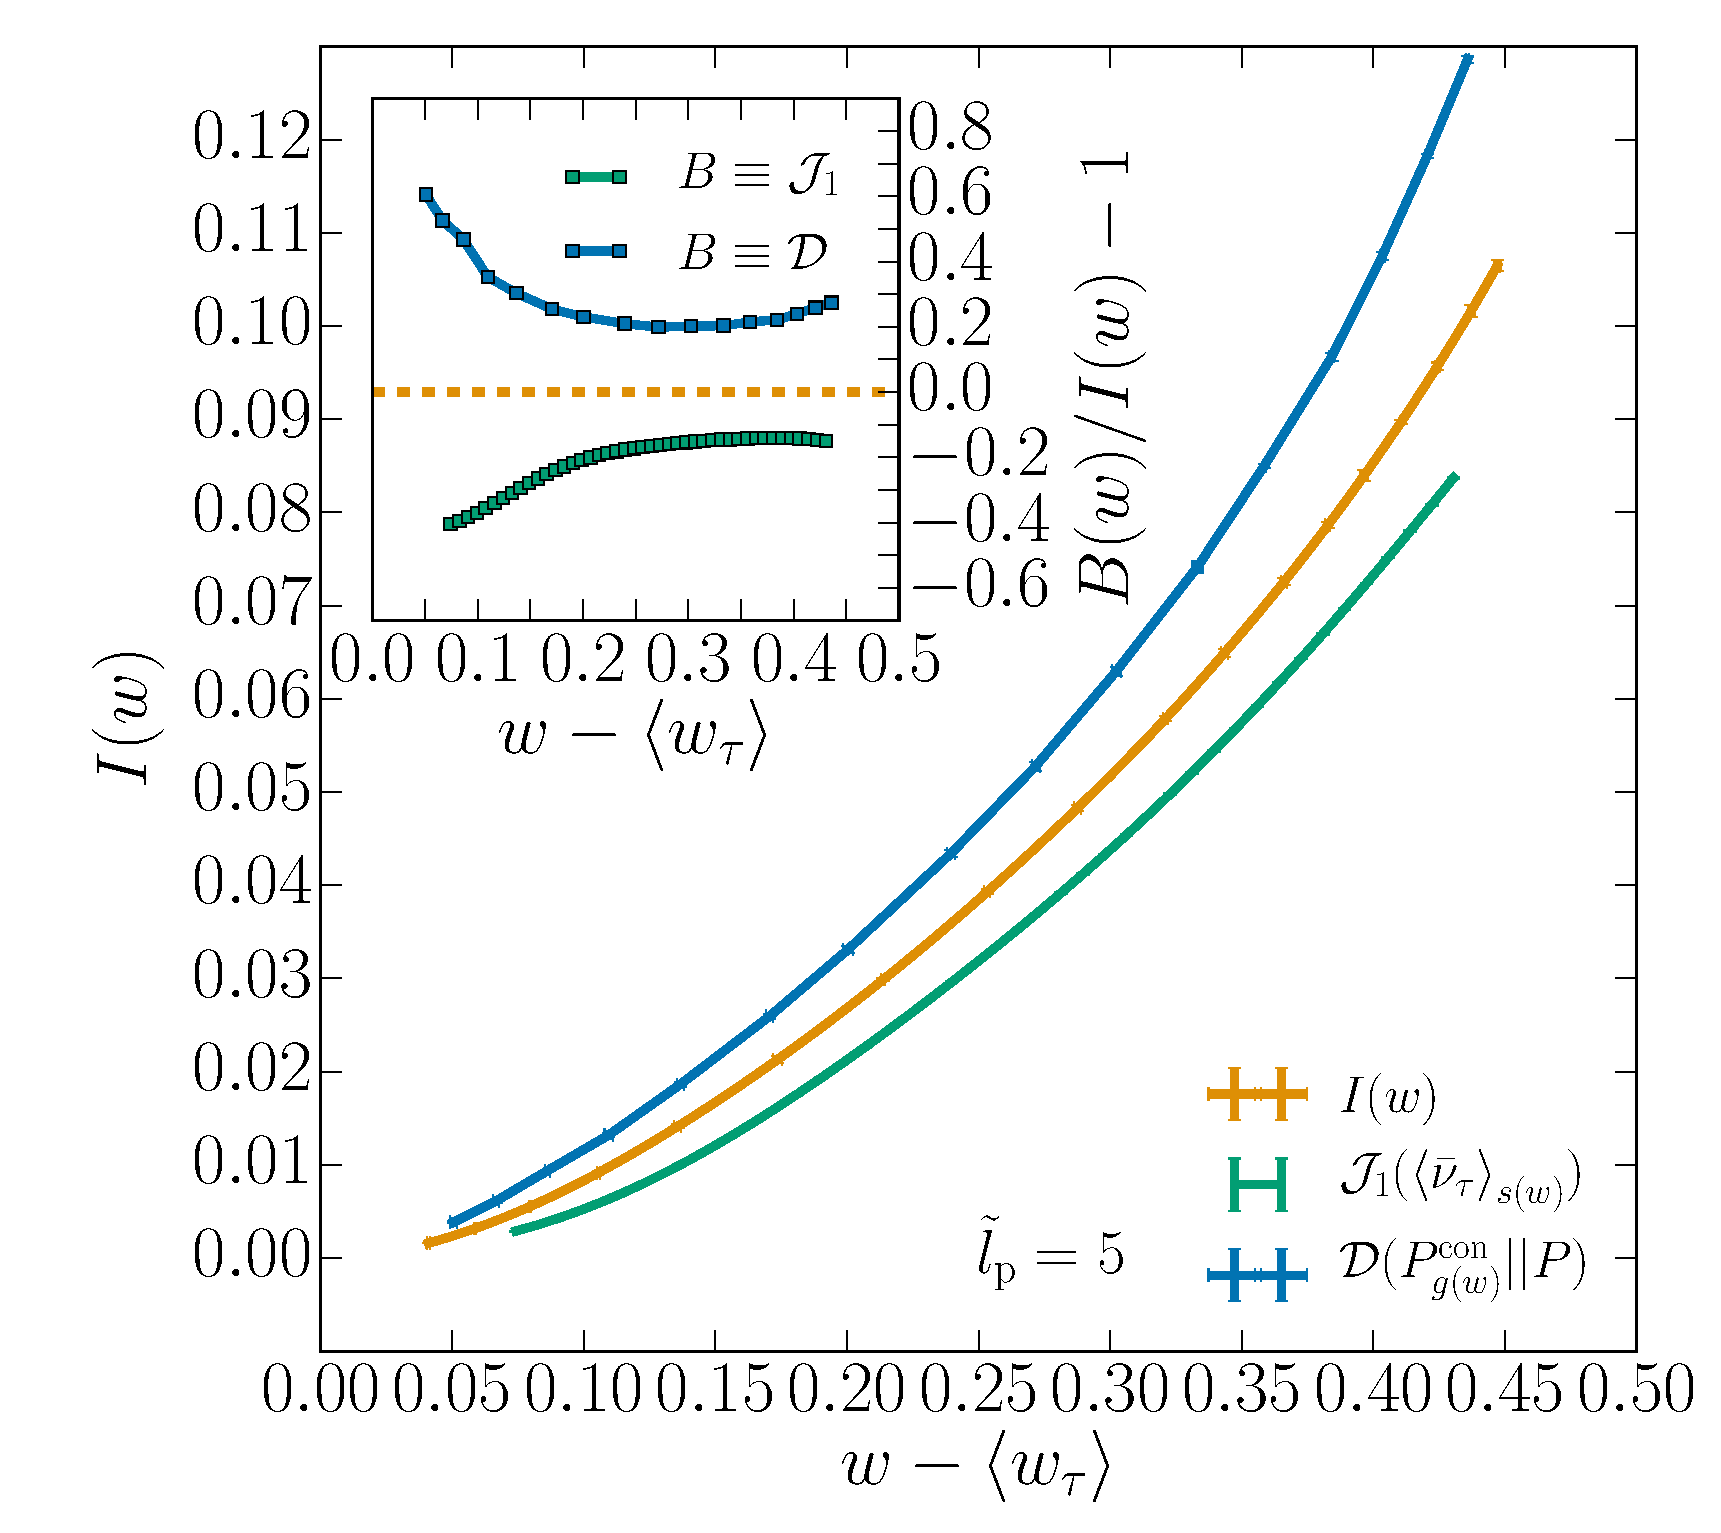
\includegraphics[width=0.45\textwidth]{boundRate.eps}
\includegraphics[width=0.45\textwidth]{boundRate40.eps}
\caption{Bounds to the rate function $I(w)$. \FigureFrom{keta2020collective}{}}
\end{figure}

\begin{itemize}
  \item {\bf $w > w^*$ (CM):} fluctuations of $w_{\tau}$ strongly coupled to those of $\bar{\nu}_{\tau}$
  \item {\bf $w < w^*$ (isotropic):} $w_{\tau}$ is enhanced by other mechanisms than orientation coupling
\end{itemize}

\end{frame}

\begin{frame}{Density fluctuations}

\vspace{-10pt}
\begin{align*}
S_s(\boldsymbol{q}) = \left<\rho_{\boldsymbol{q}} \rho_{-\boldsymbol{q}}\right>_s
\end{align*}

\begin{figure}
\centering
\includegraphics[width=0.80\textwidth]{S_Nn1000_Dk6500_Ll5000_NCo1000.eps}
\caption{Biased structure factor $S_s$. \FigureFrom{keta2020collective}{}}
\end{figure}

\begin{itemize}
  \item[$\rightarrow$] small-$q$ limit not apparent
  \item[$\Rightarrow$] density fluctuations suppressed for $s < 0$
\end{itemize}

\end{frame}

\subsection{Passive limit}

\begin{frame}{High $D_r$}

\vspace{-5pt}

\begin{figure}
\centering
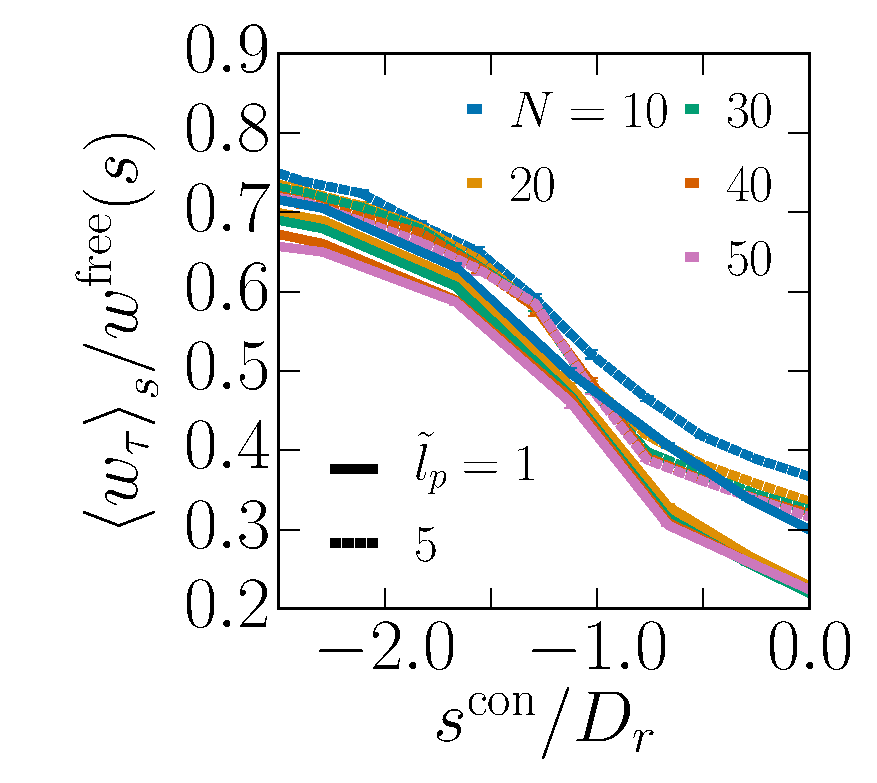
\includegraphics[width=0.30\textwidth]{sWork_N_Dk6500_Tn1000-Ll1000-con.eps}
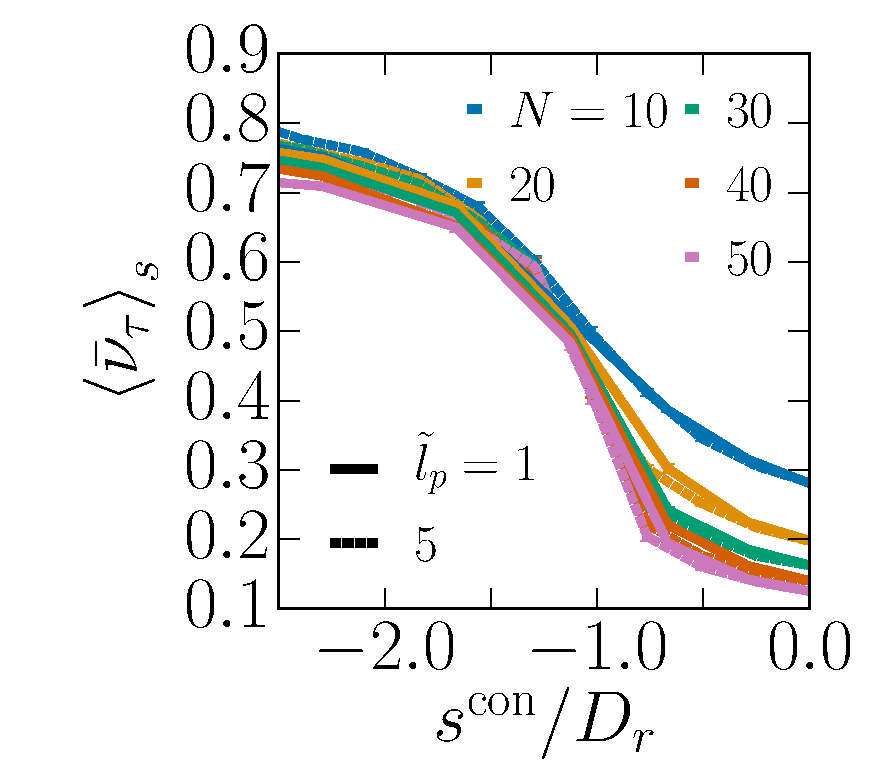
\includegraphics[width=0.30\textwidth]{sOrder_N_Dk6500_Tn1000-Ll1000-con.eps}\\
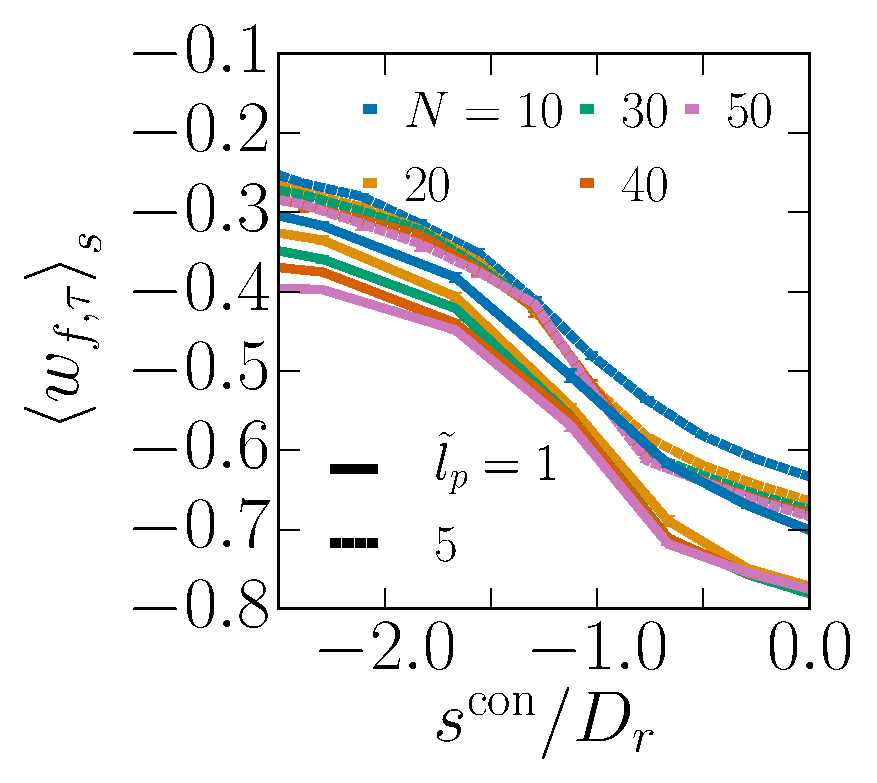
\includegraphics[width=0.30\textwidth]{sWorkForce_N_Dk6500_Tn1000-Ll1000-con.eps}
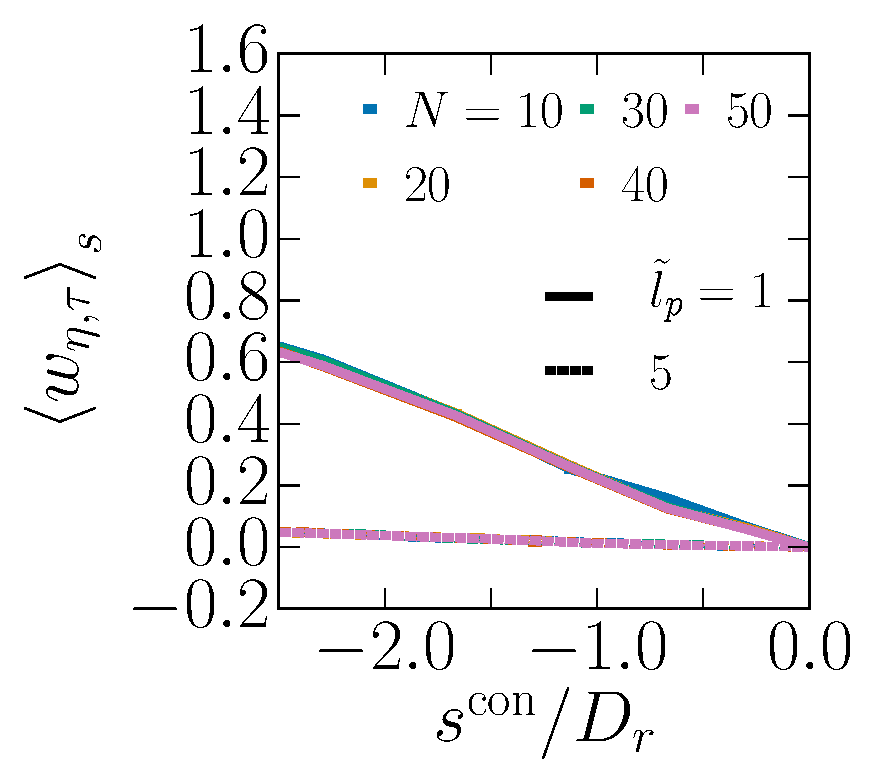
\includegraphics[width=0.30\textwidth]{sWorkNoise_N_Dk6500_Tn1000-Ll1000-con.eps}
\vspace{-5pt}
\caption{Biased averages of the polarisation $\left<\bar{\nu}_{\tau}\right>_s$, the active work $\left<w_{\tau}\right>_s$ and its force $\left<w_{f, \tau}\right>_s$ and noise part $\left<w_{\eta, \tau}\right>_s$. \FigureFrom{keta2020collective}{}}
\end{figure}

\begin{itemize}
  \item[$\rightarrow$] isotropic mechanism to produce large deviations of $w_{\tau}$
\end{itemize}

\end{frame}

\end{document}
